\documentclass{article}
\usepackage{listings}
\usepackage{amsmath}
\usepackage{graphicx}
\usepackage{float}
\usepackage{subcaption}
\usepackage[linewidth=1pt]{mdframed}
\usepackage[colorlinks]{hyperref}

\usepackage{algorithm}
\usepackage{algpseudocode}

\hypersetup{citecolor=DeepPink4}
\hypersetup{linkcolor=DarkRed}
\hypersetup{urlcolor=Blue}

\usepackage{cleveref}

\setlength{\parindent}{1em}
\setlength{\parskip}{1em}
\renewcommand{\baselinestretch}{1.0}

\begin{document}

\begin{titlepage}
	\centering
	{\scshape\LARGE Assignment 1\par}
	\vspace{1cm}
	{\scshape\Large Bioinformatics (CIS 455)\par}
	\vspace{1.5cm}
	{\Large\itshape Javier Arechalde\par}
	\vfill
	{\large \today\par}
\end{titlepage}

\section*{Problem 1-1 Jones \& Pevzner, Problem 2.1}
  
\subsection*{1.}

We are going to write the pseudocode for an algorithm, that given a list of $n$ numbers, returns the largest and smallest number in that list.

\begin{algorithm}[H]
\caption{Finding largest and smallest numbers}
\begin{algorithmic}[1]
\State Initialize $max$ to $L[0]$ and $min$ to $L[0]$
\For {$n$ in number list L}
 \If{$n<min$}
  \State $min = n$
 \EndIf 
 \If{$n>max$}
  \State $max = n$
 \EndIf
\EndFor
\State Return $max$ and $min$
\end{algorithmic}
\end{algorithm}

The time complexity of my algorithm will be $O(n) = n$, and the running time will be $2(n-1)+2$ because for every number in the list that starts from the second position after initialization, we need to check if the number is greater than the current maximum, or smaller than the current minimim.

\subsection*{2.}

Now we will implement an algorithm that performs only $3n/2$ comparisons to find the smallest and largest numbers in the list. For this implementation we will use the tournament method described below (Divide \& Conquer).

\begin{algorithm}[H]
\caption{Divide \& Conquer pseudocode}
\begin{algorithmic}[1]
\State We have a list $l$ with $n$ integers $l = (l_1,l_2,...l_n)$
\Function{findmaxmin}{list,alow,ahigh}
 \If{$length list = 1$}
  \State Maximum and minimum are the same

  \Return maximum and minimum
 \EndIf
 \If{$length list = 2$}
  \State Compare both elements in the list to find the maximum and minimum

  \Return maximum and minimum
 \EndIf
 \State Divide the array in half, and store the two halves in arrL and arrR
 \State Call findmaxmin to find the maximum and minimum of arrL and arrR
 \If{Maximum of arrL or arrR is greater than the current max}
  \State Update global maximum
 \EndIf
 \If{Minimum of arrL or arrR is smaller than the current min}
  \State Update global minimum
 \EndIf
 \Return the global maximum and the global minimum
\EndFunction
\State In the end, we have the maximum and minimum of the given list of integers.
\end{algorithmic}
\end{algorithm}

In this case, we will divide the initial list with $n$ numbers into two lists of $n/2$ each, for eacg of this lists, we will need to find the maximum and minimum of this lists, which can be done in $n/2-1$ comparisons. So in total we will need $3n/2-2$ comparisons to find the maximum and minimum of a list containing $n$ numbers.

\section*{Problem 1-2 Jones \& Pevzner, Problem 2.2}

Now we will write the pseudocode for two algorithms that iterate over every index from $(0,0,...,0)$ to $(n_1,n_2,...,n_d)$, one of them will be recursive and the other one iterative.

\subsection*{Iterative pseudocode:}

\algnewcommand\algorithmicforeach{\textbf{for each}}
\algdef{S}[FOR]{ForEach}[1]{\algorithmicforeach\ #1\ \algorithmicdo}

\begin{algorithm}[H]
\caption{Iterative pseudocode}
\begin{algorithmic}[1]
\State We have two indexes lists $l = (0,0,...0)$ and $n = (n_1,n_2,...n_d)$.
\State We will print all the possible combination of elements
\ForEach{$(i_1,i_2,..,i_d)$ \textbf{from} $(0,0,...,0)$ \textbf{to} $(n_1,n_2,...,n_d)$}
  \State Return list $i$.
\EndFor
\end{algorithmic}
\end{algorithm}

\subsection*{Recursive pseudocode:}

\begin{algorithm}[H]
\caption{Recursive pseudocode}
\begin{algorithmic}[1]
\State We have two indexes lists $l = (0,0,...0)$ and $n = (n_1,n_2,...n_d)$.
\State We will recursively build a tree to print all the possible combinations
\Function{Combinations}{n,lev,index}
\While{lev<d}
 \State Add n_index to list $list$
 \If{level=0}
  \State Return array of 0's
 \EndIf
 \If{index = d}
  \State Reset index
 \EndIf
 \If{We reach the lenght of l and used all d}
  \State Go down one level and reset index
 \EndIf
\For{$n_i$ in $n$}
\State Return ()
\Call{Combinations}{n,lev,i}
\EndFunction
\State Return the $sum$ value
\end{algorithmic}
\end{algorithm}

\section*{Problem 1-3 Jones \& Pevzner, Problem 2.3}

\begin{itemize}

\item Yes, $\log n = O(n)$, because $O(n)$ is an upper bound for $\log n$, as it grows faster.

\item No, $\log n = \Omega(n)$, because $\Omega(n)$ is not a lower bound for $\log n$, as $\log n$ grows significantly slower.

\item No, $\log n = \Theta(n)$, because $\log n$ is not $O(n)$ and $\Omega(n)$ at the same time.

\end{itemize}

\section*{Problem 1-4 Jones \& Pevzner, Problem 2.17}

\subsection*{Will the viruses eventually kill all the bacteria?}
In order to find if the viruses end up killing all the bacteria in the Petri dish, we only need to prove that the growth rate of the viruses is higher than the growth rate of the bacteria.

In the first minute, the virus kills one bacteria, and produces another copy of himself, and all the remaining bacteria reproduce, making $2$ viruses and $2(n-1)$ bacteria.

The number of viruses continue to double at each step, also, the number of bacteria double at each step too, but before the bacteria double, the viruses kill as many bacteria as the number of viruses there are at that moment. Then, the growth rate of bacteria is slower than the growth rate of the viruses, because is slowed by the number of viruses at each step. Thus, at some point, the bacteria will be exterminated by the viruses.

\subsection*{Algorithm design}

\begin{algorithm}[H]
\caption{Algorithm for calculating the number of steps}
\begin{algorithmic}[1]
\State At the beginning we have $n_v = 1$ virus and $n_b = n$ bacteria
\State At each step, the number of viruses double, the bacteria double too, but $n_v$ are killed by the virus too before they double.
\While {$n_b>n_v$}
 \State $n_b = 2*(n_b-n_v)$
 \State $n_v = 2*n_v$
 \State $steps++$
\EndWhile
\end{algorithmic}
\end{algorithm}

\section*{Problem 1-5}

\begin{figure}[H]
\begin{center}
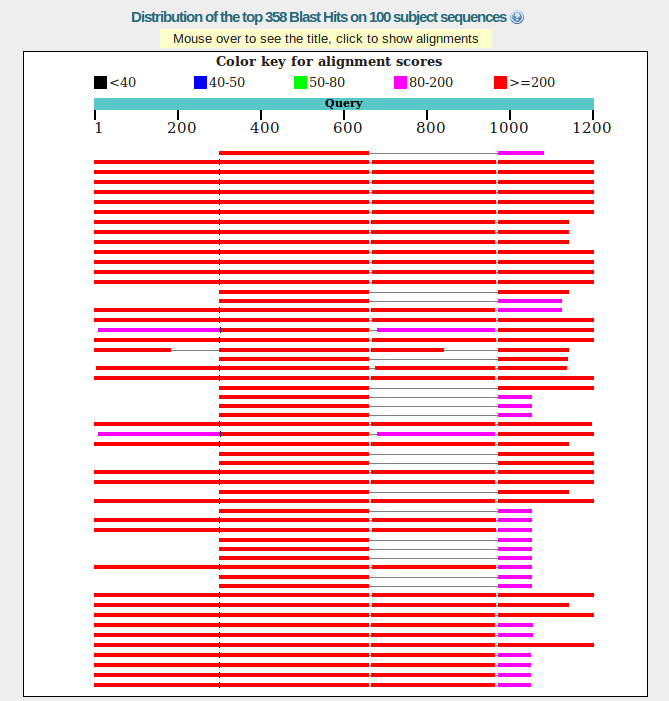
\includegraphics[scale = .4]{Dinosaur}
\end{center}
\caption{DNA Sequence}
\end{figure}

\subsection*{5.A}
The highest total score is $3599$ with a max score of $435$.

\subsection*{5.B}
The description of the result with the highest score is: \textit{Cloning vector pAxCALRL, complete sequence}.

\subsection*{5.C}
The query coverage of this result is: $99\%$

\subsection*{5.D}
The DNA sequence in Jurassic Park is \textbf{fictional}, because the tool we used couldn't find a match without gaps in the database. The lowest fraction of gaps found was $12\%$, that's why the maximum Ident value is $88\%$.

\section*{Problem 1-6 Rosalind}

\end{document}
